% vim: set tw=0:
\documentclass{beamer}
\usepackage{graphicx}

% Reasonable themes:
% Antibes Bergen Berkeley Berlin Frankfurt Goettingen Ilmenau Luebeck Malmoe
% Montpellier PaloAlto Rochester Singapore Szeged Warsaw bars boxes
% compatibility default lined plain shadow sidebar split tree
% And these ones include the author's name on every slide:
% Berkeley

% Declare themes.
\mode<presentation>
\usetheme{UWHEP}

% Personal macros.
\newcommand{\email}[1]{{\texttt #1}}
\newcommand{\newframe}[1]{\section{#1}
    \frametitle{\sc{#1}}}
\newcommand{\subframe}[1]{\subsection{#1}
    \frametitle{\sc{#1}}}
\newcommand{\supers}[1]{\ensuremath{^\textrm{#1}}}
\newcommand{\subs}[1]{\ensuremath{_\textrm{#1}}}
\newcommand{\ca}{\ensuremath{\sim}}

% Author information.
\title{T2 Status}
\author[Maier, Mohapatra]{
    Will Maier \and Ajit Mohapatra\\ 
    {\tt wcmaier@hep.wisc.edu}\\
    {\tt ajit@hep.wisc.edu}}
\institute[Wisconsin]{University of Wisconsin - High Energy Physics}
\date{2008.03.18}
\logo{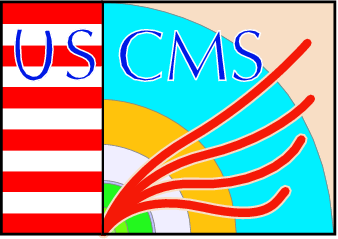
\includegraphics[height=0.6cm]{../../../Graphics/USCMS_logo.png}\hspace{.1cm}
\includegraphics[height=0.75cm]{../../../Graphics/UW_logo.png}}

\begin{document}

\begin{frame}
    \titlepage
\end{frame}

%\section{Overview}
%\begin{frame}
%    \tableofcontents
%\end{frame}

% http://indico.cern.ch/conferenceDisplay.py?confId=30680
% http://evo.caltech.edu/evoGate/koala.jnlp?meeting=e9eIeivIvuaealIIaaI9
% 626 395 2112 / 267162

\section{Facilities}
\subsection{Software and Storage}
\begin{frame}
\frametitle{}
\begin{itemize}
    \item 2008 Deployment plans
    \begin{itemize}
        \item 32 dual-quad Xeon E5450 (3.0 GHz) in Supermicros
        \item 4x1TB disks, 16GB RAM in each node
        \item Total: 128 TB, 256 cores, \$156,000
        \item Considered Sun quote (but not enough TB/1U)
        \item Will hopefully send order this week
    \end{itemize}
    \item High level of local analysis in the last few weeks
    \item Scattered crashes due to CMSSW size; not enough to tighten memory requirements
    \item Upgraded opportunistic resources to Condor 7.0.1
    \item PFM performing well
    \begin{itemize}
        \item Oddly, a failed node caused slow downs in some dCache operations (PoolManager, admin interface)
        \item Led to several slow PFM runs; after node was shut off, PFM returned to normal
    \end{itemize}
\end{itemize}
\end{frame}

\subsection{Production and Monitoring}
\begin{frame}
\frametitle{}
\begin{itemize}
    \item SAM: OK
    \item JobRobot: OK
    \item LoadTest:
    \begin{itemize}
        \item Exercising links under DDT2
        \item CERN, CNAF, FNAL links commissioned; exercising FZK link
        \item Regular subscription of MC data for local users
    \end{itemize}
    \item MC Production:
    \begin{itemize}
        \item Last bits of CSA07 signal production in OSG with a seven month old ProdAgent
        \item Updating to the latest PA release and testing many updates for CSA08 production
    \end{itemize}
\end{itemize}
\end{frame}
\end{document}
